\documentclass{beamer}
\graphicspath{{../graphics/}}
\usepackage{listings}
\usepackage{ulem}
\usepackage{subcaption}
\captionsetup{compatibility=false}
\usepackage{algorithm2e}

\newcommand{\linespace}{\vspace{1em}}

\mode<presentation>
{
  \usetheme{Darmstadt}
  \setbeamertemplate{footline}[frame number]
  \setbeamertemplate{navigation symbols}{}
  \setbeamercovered{transparent}
}

\AtBeginSection[]
{
   \begin{frame}
        \frametitle{Indhold}
        \tableofcontents[sectionstyle=show/hide,subsectionstyle=show/show/hide]
   \end{frame}
}

%\usepackage[danish]{babel}
\usepackage[T1]{fontenc}

\usepackage[utf8]{inputenc}

\usepackage{times}

\usepackage{tikz}
\usepackage{3dplot}
\usepackage{multirow}

\title[Mapping med Lego-robot]{Mapping med Lego-robot}

\subtitle{SW505E13}

\author[SW505E13]{Mikkel Sand\o ~Larsen, \and Bruno Thalmann, \and Stefan Marstrand Getreuer Micheelsen, \and Stefan Thilemann, \and Mikael Elki\ae r Christensen, \and Anders R. Nielsen}

\institute[Aalborg University]
{
  Department of Computer Science\\
  Aalborg University}

\date[CFP 2003]{31. Januar 2014}

\begin{document}

%--------------------------------------------------
%     INTRODUKTION
%--------------------------------------------------

\begin{frame}
  \titlepage
\end{frame}

\begin{frame}
    \frametitle{Indhold}
    \tableofcontents[sectionstyle=show/show,subsectionstyle=hide/hide/hide]
\end{frame}

\section{Overblik}

%--------------------------------------------------
%     BAGGRUND
%--------------------------------------------------
\subsection{Baggrund}
\begin{frame}[fragile]{Anvendelse}
	Stort anvendelsesområde for robotter
	\begin{itemize}
		\item Industri
			\begin{itemize}
			\item Droner (overvågning/kortlægning)
			\item Lager robotter
			\end{itemize}
		\item Privat
			\begin{itemize}
			\item Støvsuger robotter
			\item Plæneklipper robotter
		\end{itemize}
	\end{itemize}
\end{frame}

\begin{frame}[fragile]{Grundlæggende problemstillinger}
	\begin{columns}
		\begin{column}{0.5\textwidth}
			Krav til robotten så den kan begå sig i dens omgivelser
			\linespace
			\begin{itemize}
				\item Lokation (interaktion med omgivelser)
				\item En form for kort (til navigation)
			\end{itemize}
		\end{column}
		\pause
		\begin{column}{0.5\textwidth}
			SLAM (\textbf{S}imultaneous \textbf{L}ocalization \textbf{A}nd \textbf{M}apping)
			\linespace
			\begin{itemize}
				\item \textit{Svært!}
					\begin{itemize}
						\item Approximering af lokation
					\end{itemize}
				\item Lokation afhængig af kort, og omvendt
			\end{itemize}
		\end{column}
\end{columns}
\end{frame}


\subsection{Problem}
%--------------------------------------------------
%     AFGRÆNSNING
%--------------------------------------------------
\begin{frame}[fragile]{Afgrænsning}
	\begin{itemize}
		\item Lokalisering vha. color-tracking fra Kinect
	\end{itemize}
	
	\linespace
	\pause
	
	Simplificering af robottens kørselsmiljø:
	\begin{itemize}
		\item Robottens verden er 90 grader
		\item Verdenen er et afgrænset område
		\item Verdenen er plan og befinder sig indendørs
	\end{itemize}
	\linespace
	Mindsker kravene til robotten og gør det nemmere at evaluere resultater.
\end{frame}

%--------------------------------------------------
%     PROBLEMFORMULERING
%--------------------------------------------------
\begin{frame}[fragile]{Problemformulering}
	\begin{center}
		\textit{Hvordan kan der konstrueres software til en robot, hvis formål er at kortlægge en ukendt verden, forudsat at den til enhver tid kender sin position?}
	\end{center}
\end{frame}

%--------------------------------------------------
%     MÅLSÆTNING
%--------------------------------------------------
\begin{frame}[fragile]{Målsætning}
	Grundlag for evaluering af det endelige produkt:
	\begin{itemize}
	\item To forskellige overvejelser
		\begin{itemize}
			\item Hastighed af kortlægning
			\item Præcision af kortlægning
		\end{itemize}
	\end{itemize}
	\linespace
	\pause
	
	Målet med dette projekt:
	\begin{itemize}
		\item At bygge en robot, der kan konstruere et præcist kort
	\end{itemize}
	\linespace
	\pause
	
	Vurdering af valgte målsætning:
	\begin{itemize}
		\item \textit{Det skal være muligt at navigere alene ud fra informationen i kortet og køre fra et hjørne til det diagonalt modsatte}
	\end{itemize}
\end{frame}

%--------------------------------------------------
%     FORSØGSOPSTILLING
%--------------------------------------------------
\subsection{Forsøgsopstilling}
\begin{frame}[fragile]{Kørselsmiljø set fra siden}
	\begin{figure}
		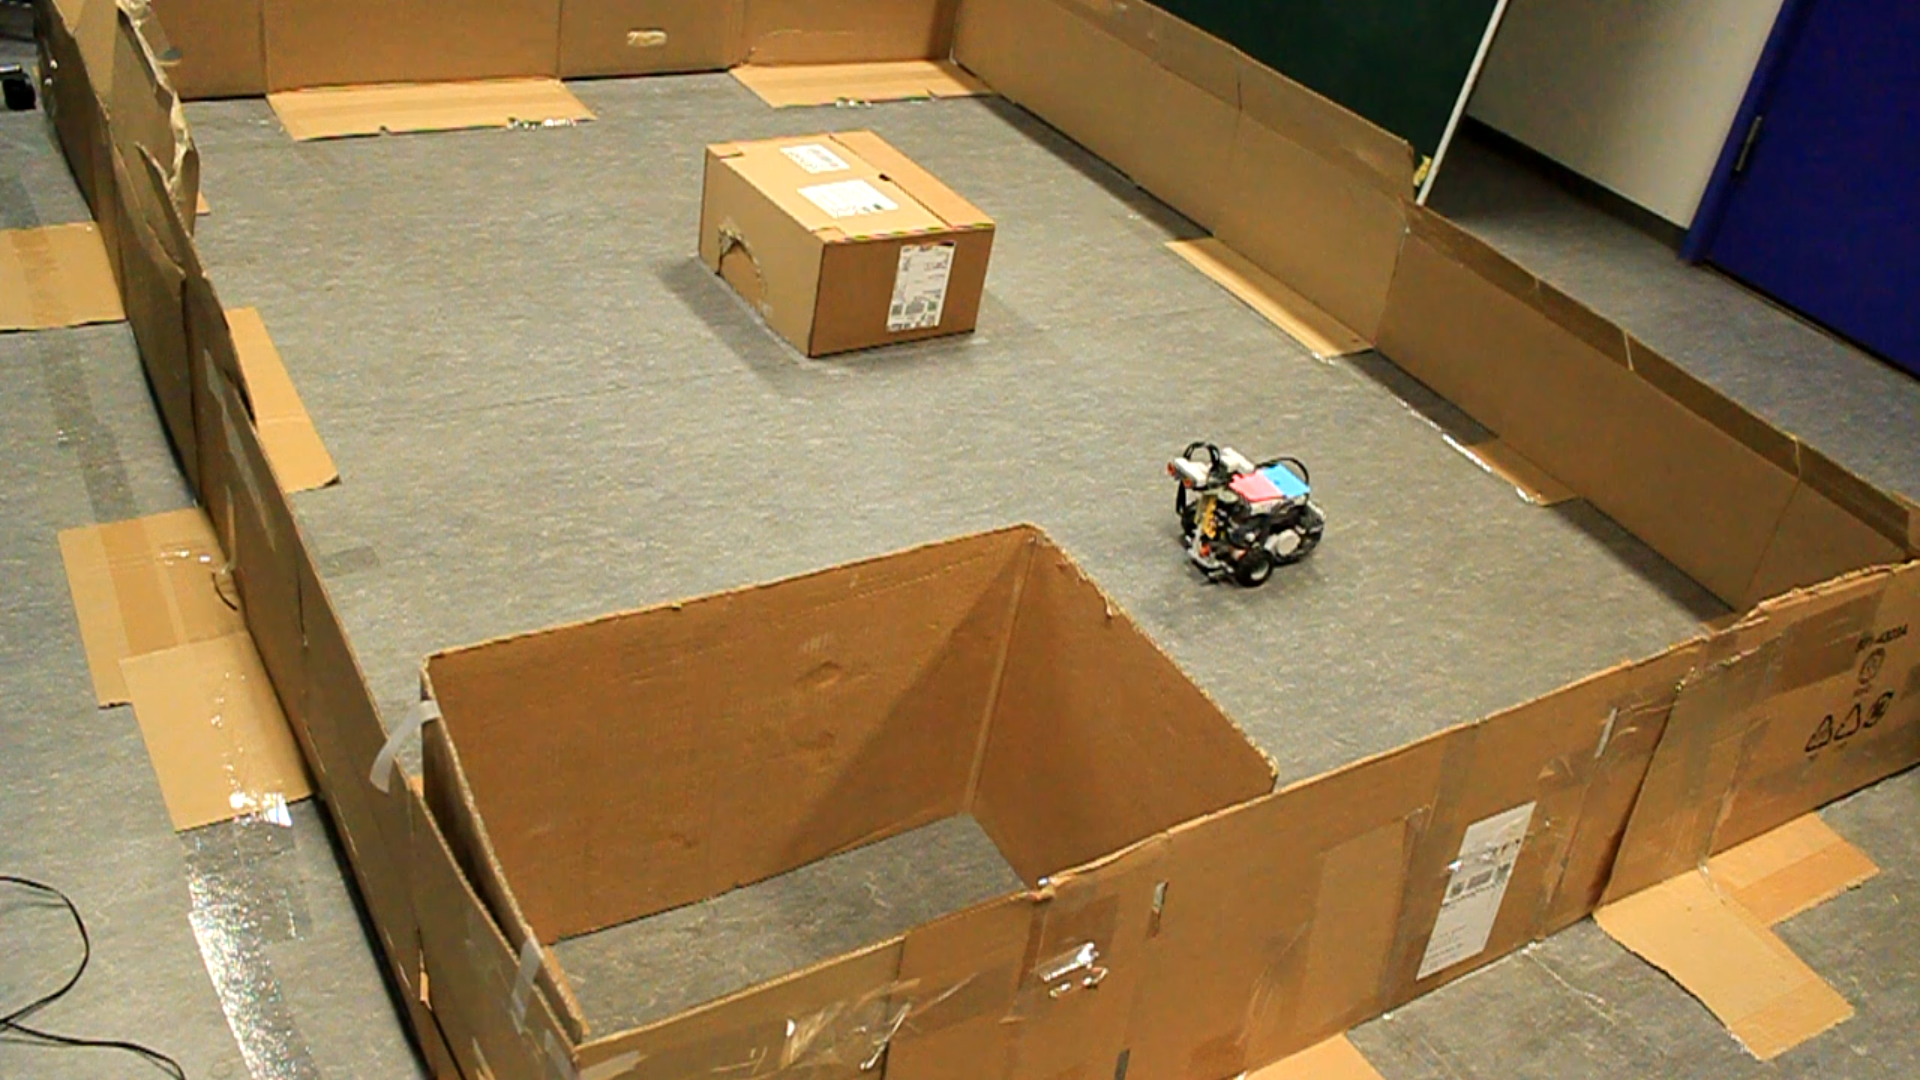
\includegraphics[width=1\textwidth]{verden/opstilling.png}
	\end{figure}
\end{frame}

\begin{frame}[fragile]{Forsøgsopstilling og Kinect}
	\begin{columns}
		\begin{column}{0.5\textwidth}
			\begin{itemize}
				\item Kørselsmiljø set fra Kinect
			\end{itemize}
			\begin{figure}
				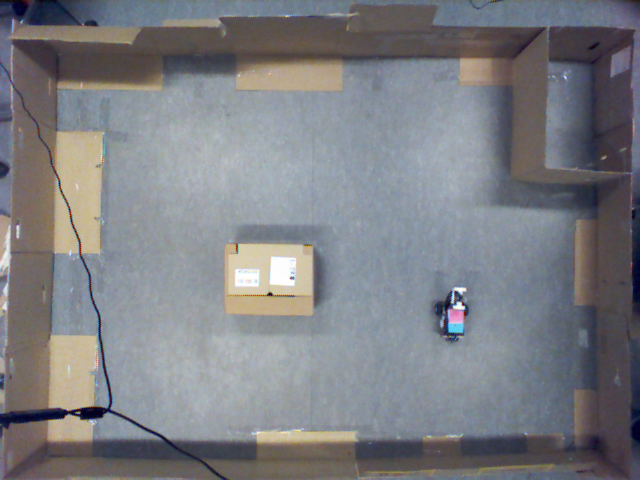
\includegraphics[width=1\textwidth]{evaluering/emptyGrid.png}
			\end{figure}
		\end{column}
		
		\begin{column}{0.5\textwidth}
				\begin{itemize}
					\item Montering af Kinect i loft
				\end{itemize}
			\begin{figure}
				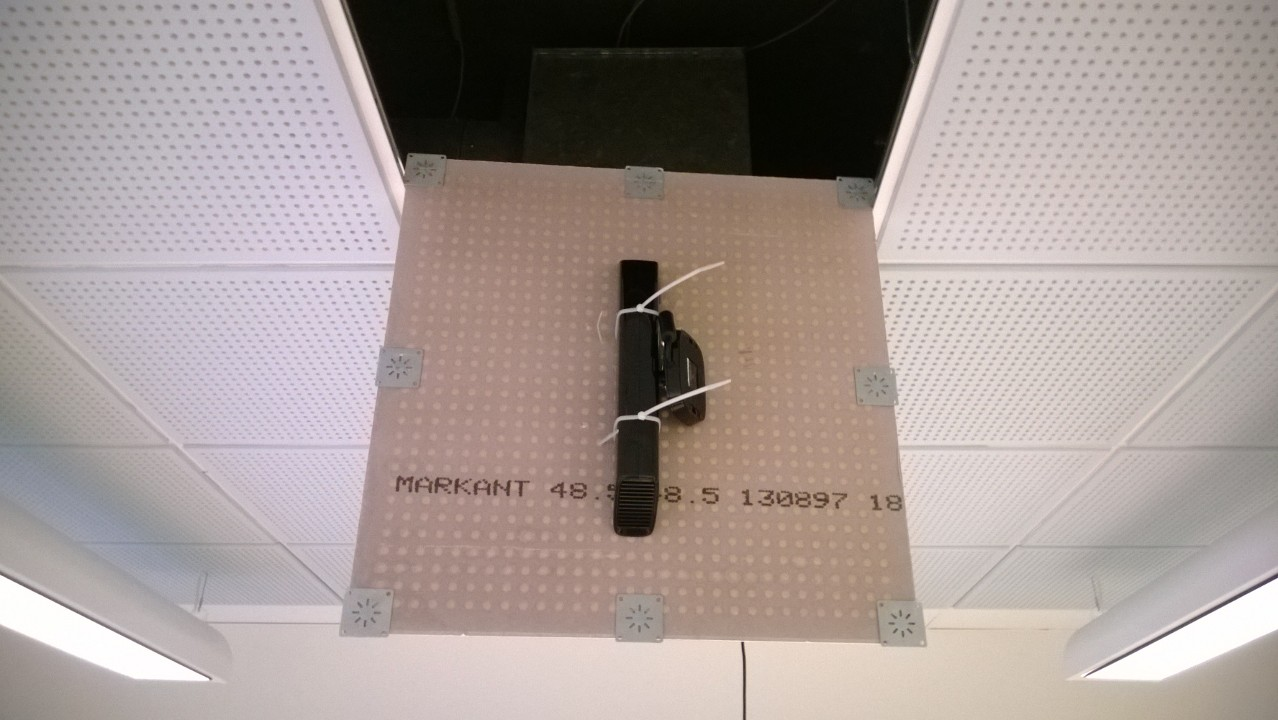
\includegraphics[width=1\textwidth]{verden/kinect.jpg}
			\end{figure}
	\end{column}
\end{columns}
\end{frame}

%--------------------------------------------------
%     EVALUERINGSMETODE
%--------------------------------------------------
\subsection{Evaluering af målsætning}
\begin{frame}[fragile]{Vurderingsmål}
	\begin{itemize}
		\item Approximering af et optimalt kort for forsøgsopstillingen
	\end{itemize}
	
	\begin{figure}
		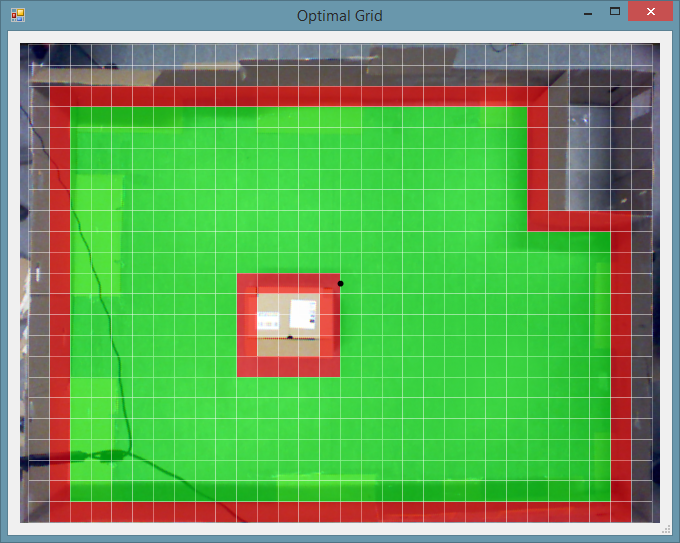
\includegraphics[width=.65\textwidth]{evaluering/optimalgrid.png}
	\end{figure}
\end{frame}

\section{Løsningsmetoder}
%Løsningsmetoder
\subsection{Platform}
\begin{frame}
\frametitle{Lego Mindstorms}
\begin{itemize}
\item Tilgængelighed
\item Nemt at gå til
\item Stort udvalg af sensorer
\item Mange muligheder ift. styring
\end{itemize}
\end{frame}

\begin{frame}
\frametitle{API}
\begin{itemize}
\item NXC
\begin{itemize}
\item NXC er et C-lignende sprog med gode indbyggede funktioner
\item NXC har gode indbyggede funktioner til fejlfinding
\end{itemize}
\item MindSqualls
\begin{itemize}
\item Et .NET bibliotek skrevet i C\#
\item Tillader nem direkte kommunikation med sensorer og motorer
\end{itemize}
\end{itemize}
\end{frame}
\subsection{Sensorer og Motor}
\frametitle{Valgt sensor og motor}
\begin{frame}
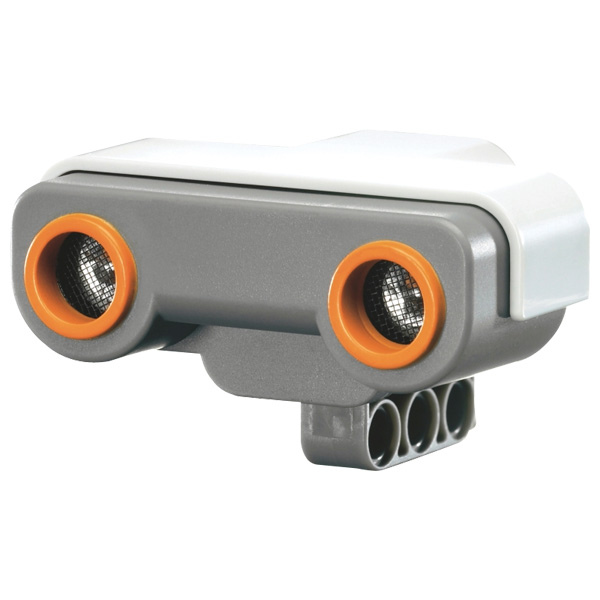
\includegraphics[width=110px, clip=true, trim = 0px 90px 0px 0px]{sensor/us}
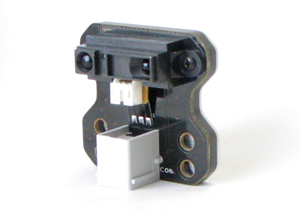
\includegraphics[width=110px]{sensor/infrared_sensor}
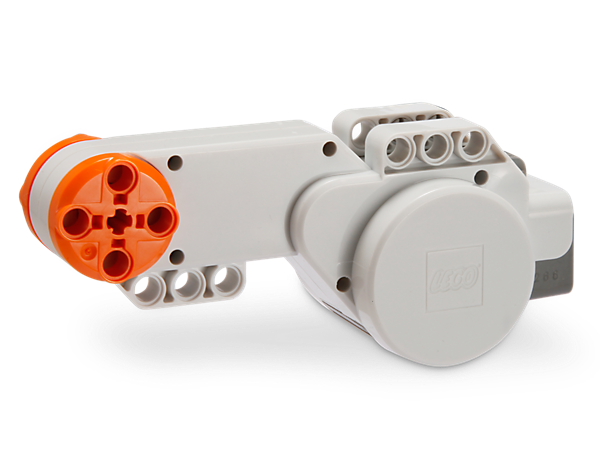
\includegraphics[width=110px]{sensor/lego_motor}
\end{frame}
\subsection{Lokalisering}
\begin{frame}
\frametitle{Valg af Kinect}
\begin{itemize}
\item Nem tilslutning til PC
\item Mange sensorer
\item Gode udviklingsværktøjer
\item Tilgængelig gennem universitetet
\end{itemize}
\end{frame}
\subsection{Mapping}
\begin{frame}
\frametitle{Occupancy grid}
\begin{itemize}
\item Til at kortlægge har vi valgt at bruge \textit{occupancy grid} algoritmen
\item \textit{Occupancy grid} er en familie af algoritmer som gør det muligt at generere konsistente kort
\item \textit{Occupancy grid} opdeler kortet i celler og tildeler en binær tilfældig variabel til hver celle
\end{itemize}
\end{frame}
%Robottens design
\section{Robottens design}
\subsection{Præsentation af designet}
\begin{frame}
\frametitle{Overordnet}
\begin{center}
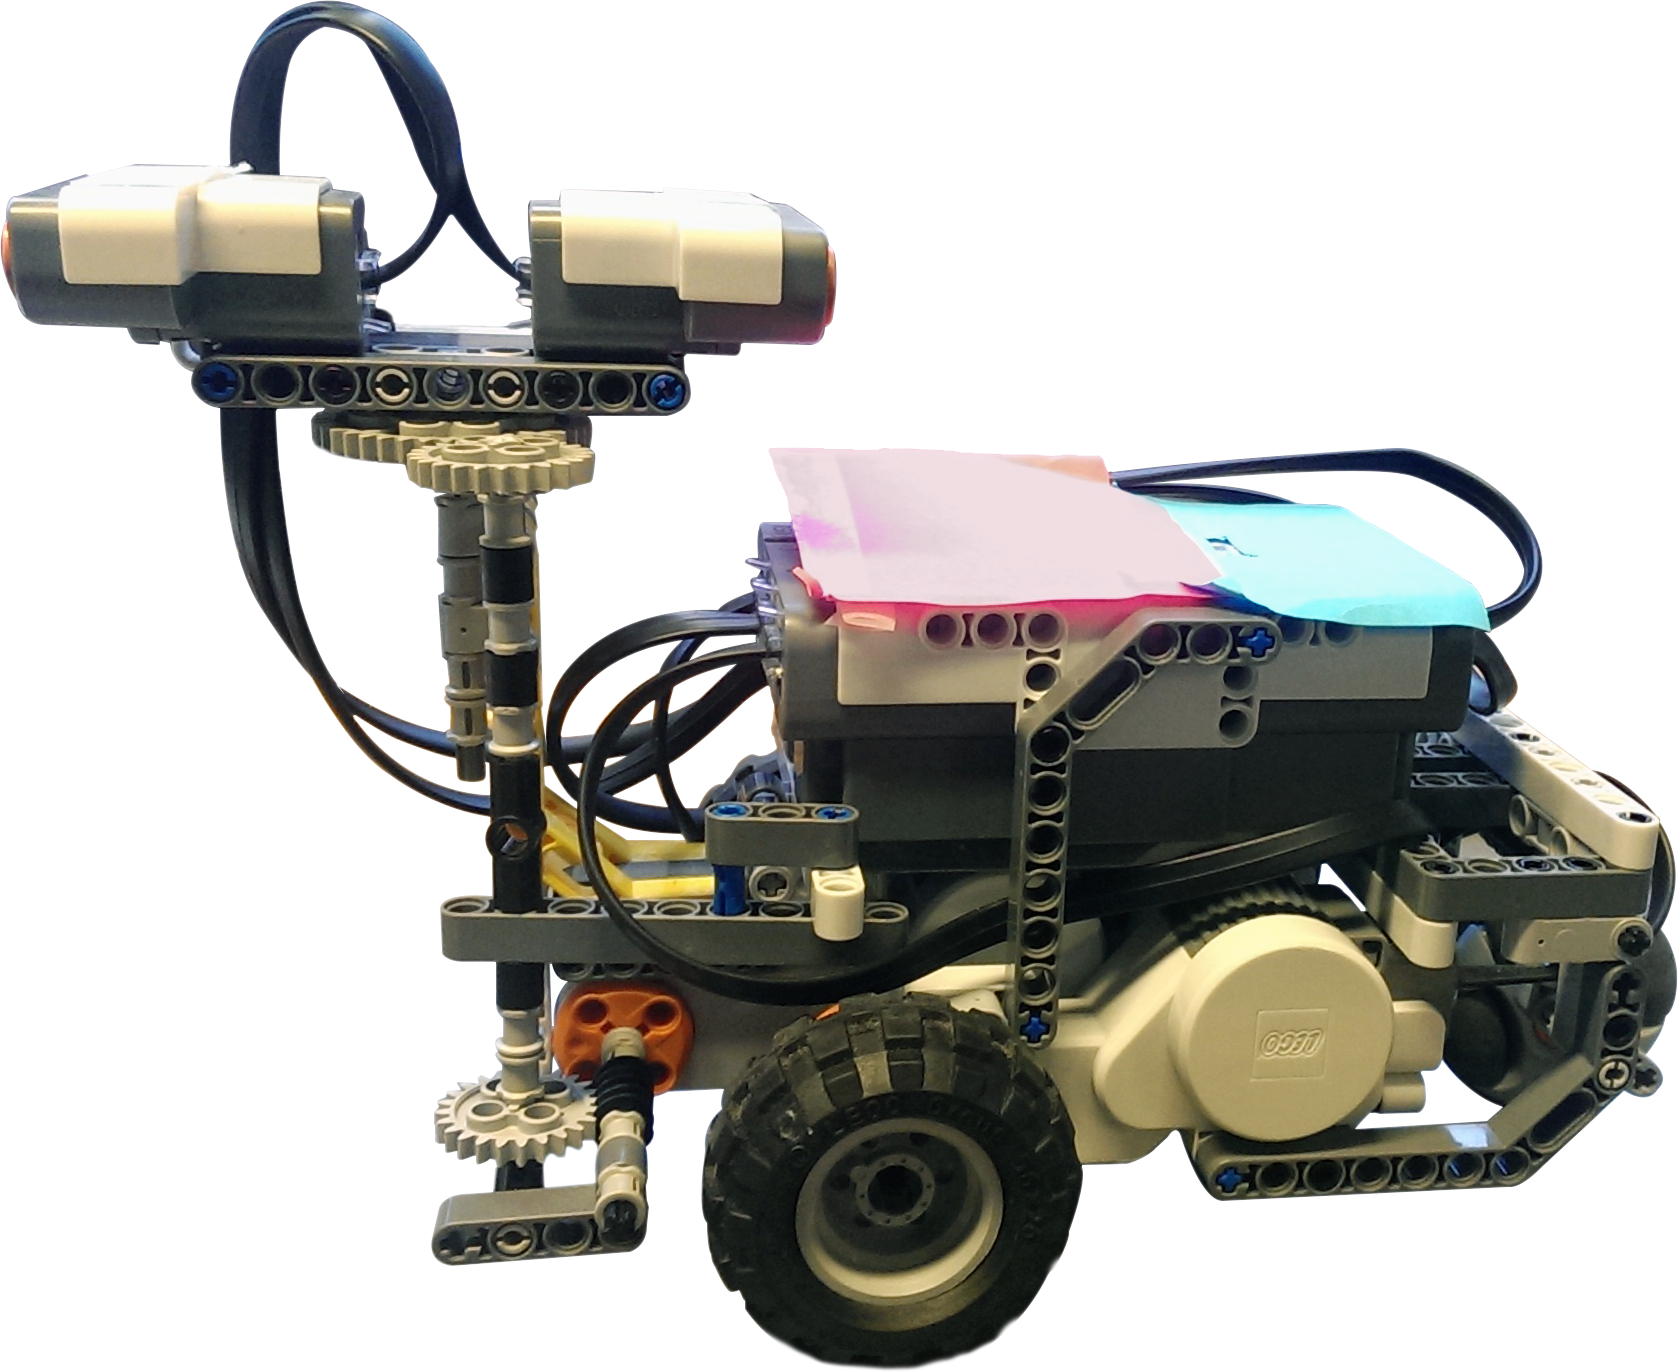
\includegraphics[scale=0.15]{whalle}
\end{center}
\end{frame}

\begin{frame}
\frametitle{Gearing}
\begin{center}
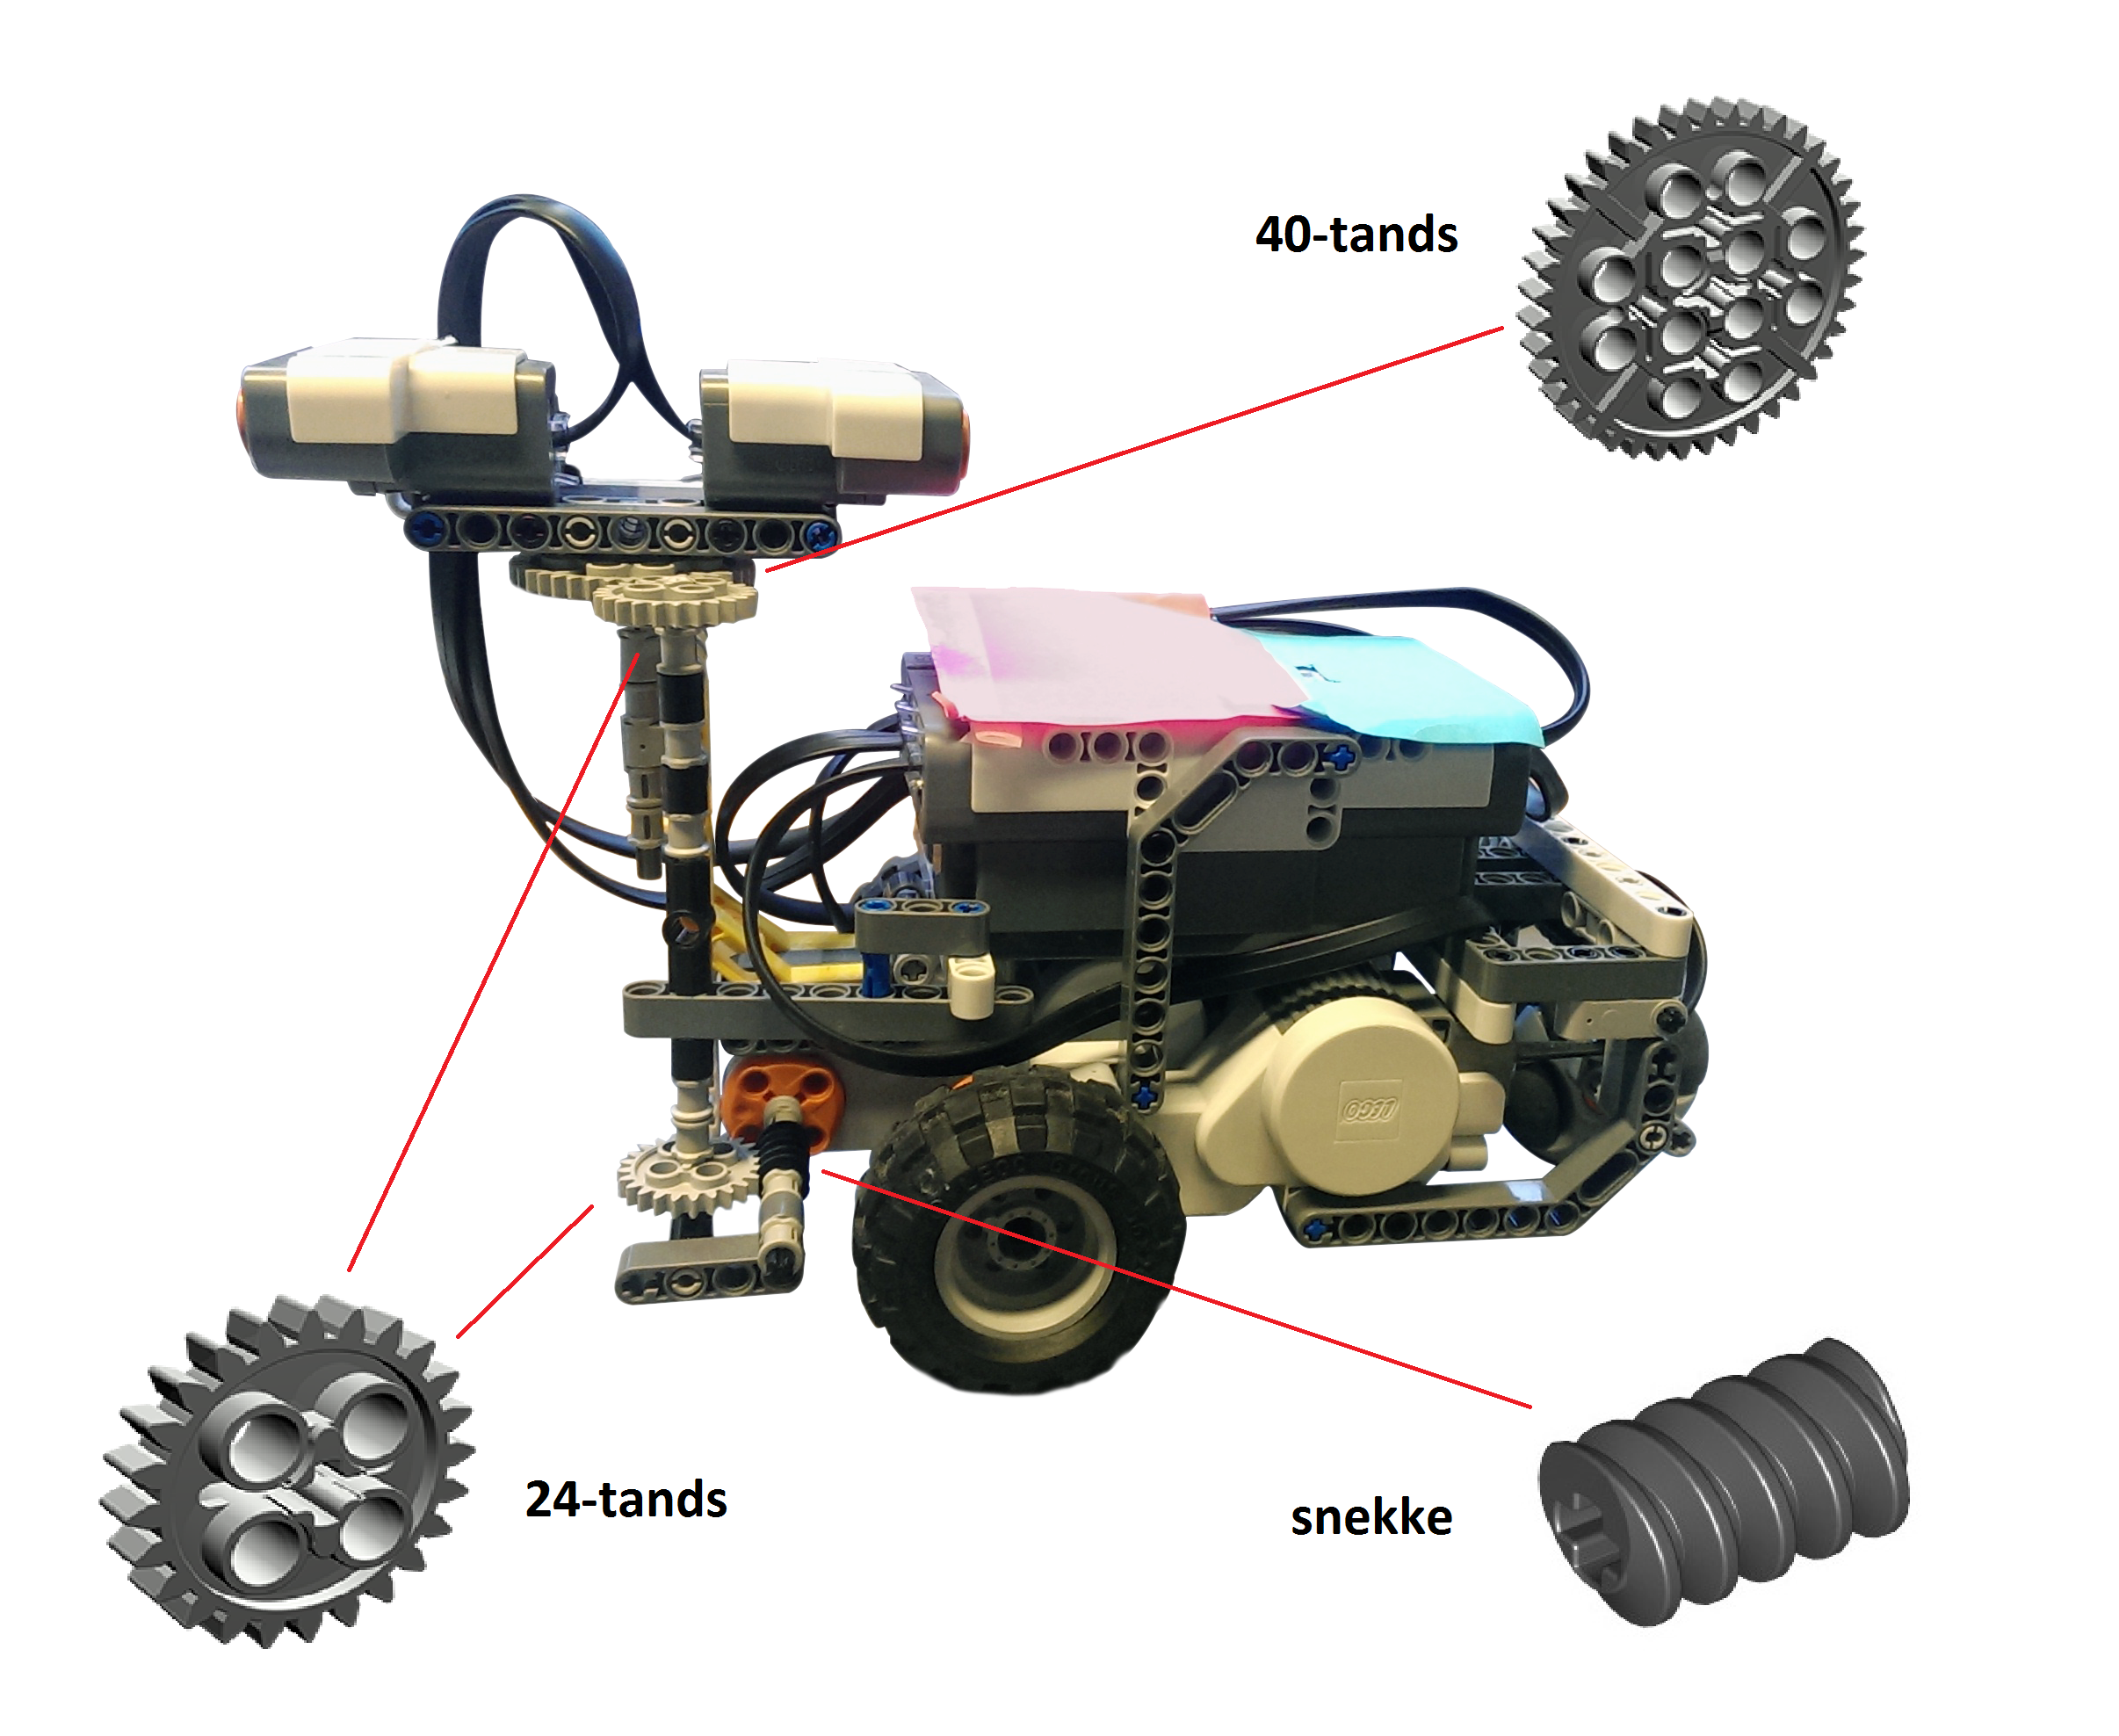
\includegraphics[scale=0.13]{whalle_with_gearing_expl}
\end{center}

\end{frame}

\subsection{Overvejelser}
\begin{frame}
\frametitle{Gearing}
\begin{itemize}
\item Gearing på hjul blev fjernet
\item Mere simpelt design
\item Unødvendigt med tårn til sensorer
\item En simplere løsning:
\begin{itemize}
\item Montere sensoren direkte på robottens krop
\item Rotere robotten når der skal måles
\end{itemize} 
\item Mindre kompleks robot design er formentlig lettere at arbejde med
\end{itemize}
\end{frame}



\section{Teori}
\subsection{Grundlæggende}
\begin{frame}{Occupancy Grid}
\begin{figure}[h] % Kørselsmiljø og et occupancy grid
\centering
	\begin{subfigure}[b]{.48\textwidth}
	\centering
	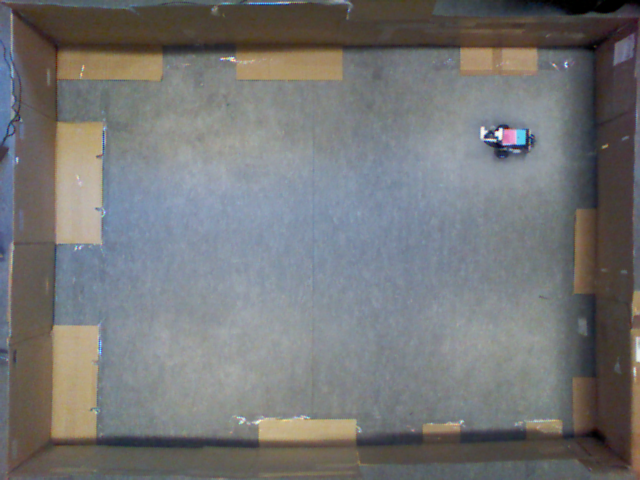
\includegraphics[width=\textwidth]{verden/oppefra_m_walle}
	\caption{Aktuelt Kørselsmiljø.}
	\label{map:world}
	\end{subfigure}
	\hfill
	\begin{subfigure}[b]{.48\textwidth}
	\centering
	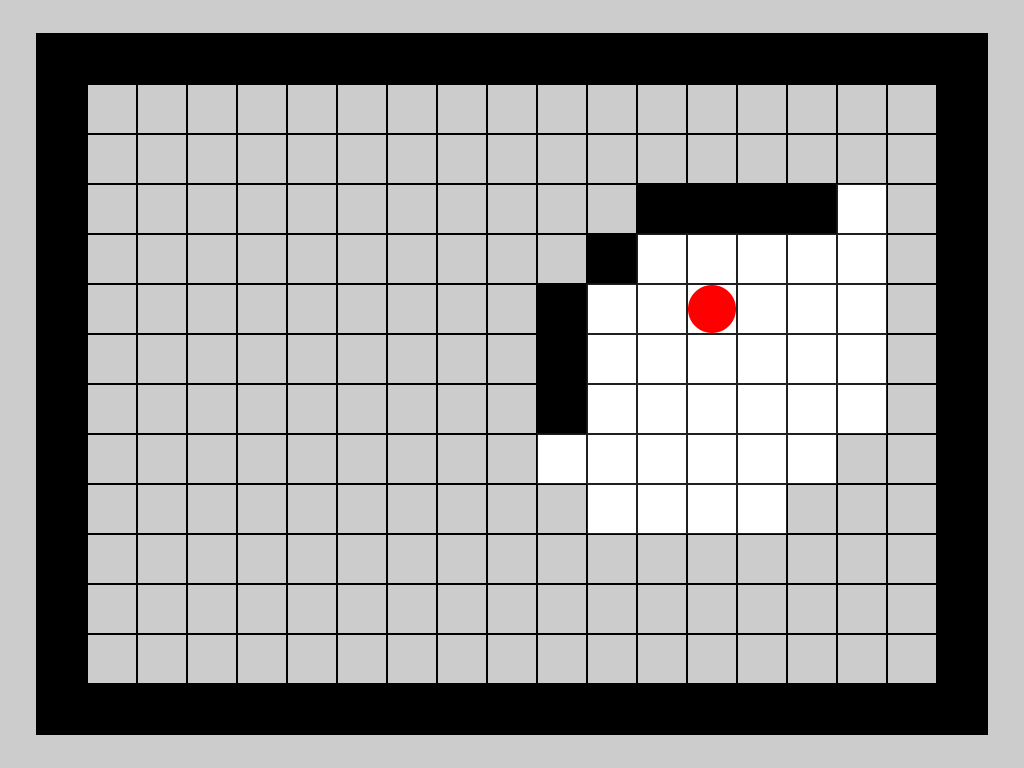
\includegraphics[width=\textwidth]{verden/occupancy_grid_verden}
	\caption{Occupancy Grid.}
	\label{map:occupancy_grid}
	\end{subfigure}

\end{figure}
\end{frame}
\begin{frame}{Bayes Regel}
Opdatering af troen på en proposition ved ny evidens
\[
\begin{split}
P(h \mid e) = \frac{P(e \mid h) \times P(h)}{P(e)}
\end{split}
\]
\end{frame}

\begin{frame}{Log Odds}
\begin{figure}
\centering 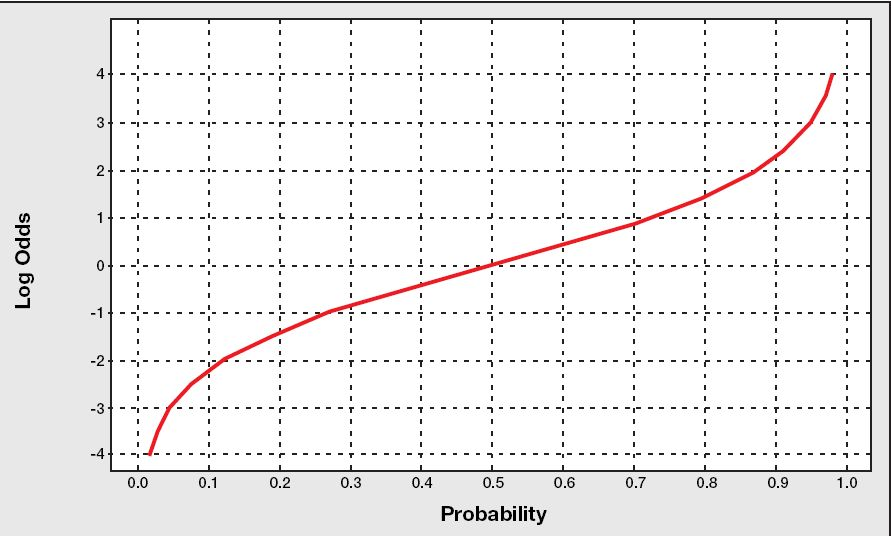
\includegraphics[scale=.2]{LogOdds}
\label{logoddsimg}
\end{figure}

%Log odds er en metode der kan benyttes for at undgå, at komponenterne i Bayes Regel enten bliver definitivt sande eller falske.
%
%Der kan derfor indføres en funktion, \textit{log odds ratio}, som mapper sandsynlighedsværdierne fra $[0;1]$ til $[-\infty;\infty]$.
%Oddset for tilstand $x$ er defineret som forholdet mellem sandsynlighederne for $x$ og $\lnot x$: 

\begin{tabular}{ p{0.5\linewidth} p{0.5\linewidth} }
$ l(x) = \log \frac{p(x)}{1 - p(x)} $ & 
$ bel_t(x) = 1 - \frac{1}{1 + exp\{l_x\}}\label{logodds:bel} $
\end{tabular}
\end{frame}

\subsection{Occupancy Grid}

\begin{frame}{Binært Bayes Filter}
Kan bruges når verdenens tilstand er statisk

\begin{algorithm}[H]
\textbf{BinaryBayesFilter($l_{t-1}, z_t$)} \\
\Indp $l_t = l_{t-1} + \log \frac{p(x \mid z_t)}{1-p(x \mid z_t)} - \log \frac{p(x)}{1-p(x)}$ \\
\Return{$l_t$}
\end{algorithm}
\end{frame}

\begin{frame}{Occupancy grid}
\begin{algorithm}[H]
OccupancyGridMapping(\{$l_{t-1,i}$\}, $x_t$, $z_t$):

\ForAll{cells $ m_i $}
{
\eIf{$ m_i $ is in the perceptual field of $ x_t $}
%then
{ $ l_{t,i} = l_{t-1,i} $ + \textbf{inverse\_sensor\_model} $( m_i, x_t, z_t ) - l_0$\\ }
%else
{ $ l_{t,i} = l_{t-1,i}  $\\ }
}
\Return {$ \{l_{t,i}\} $}
\end{algorithm}
\end{frame}

\begin{frame}{Occupancy grid}
\begin{algorithm}[H]
OccupancyGridMapping(\{$l_{t-1,i}$\}, $x_t$, $z_t$):

\ForAll{cells $ m_i $}
{
\eIf{$ x_i = x_r$ or $y_i = y_r$}
%then
{ $ l_{t,i} = l_{t-1,i} $ + \textbf{inverse\_sensor\_model} $( m_i, x_t, z_t ) - l_0$\\ }
%else
{ $ l_{t,i} = l_{t-1,i}  $\\ }
}
\Return {$ \{l_{t,i}\} $}
\end{algorithm}
\end{frame}

\subsection{Sensormodeller}
\begin{frame}{Simpel sensormodel}

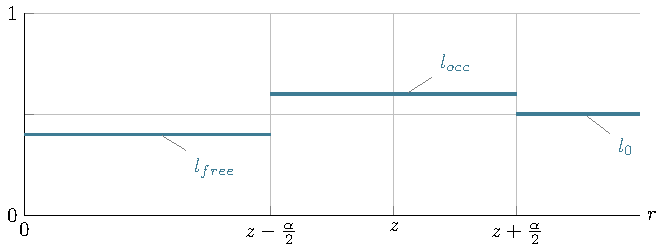
\includegraphics{simple_sensormodel.pdf}
\end{frame}

\begin{frame}{Gaussisk sensormodel}

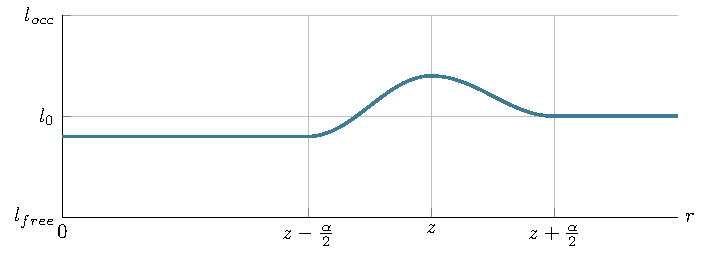
\includegraphics{gaussian_sensormodel.pdf}
\end{frame}

\begin{frame}{Sammenligning af sensormodeller}
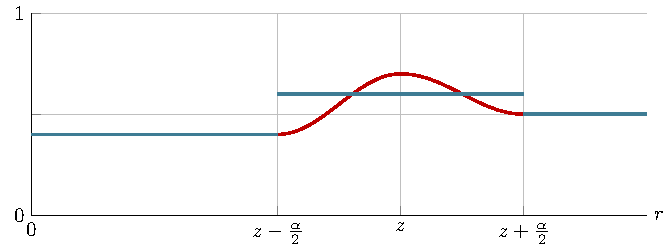
\includegraphics{combined_sensormodel}
\end{frame}


\section{Localization}

\begin{frame}{afstande mellem farver}

\centering
\tdplotsetmaincoords{60}{110}
\begin{tikzpicture}[scale=4,tdplot_main_coords]

%set up some coordinates 
%-----------------------
\coordinate (O) at (0,0,0);
\tdplotsetcoord{P1}{1.1}{60}{30}
\tdplotsetcoord{P2}{1.5}{40}{60}

%draw figure contents
%--------------------

%draw the main coordinate system axes
\draw[ultra thick,red,->] (0,0,0) -- (1,0,0) node[anchor=north east]{$r$};
\draw[ultra thick,green,->] (0,0,0) -- (0,1,0) node[anchor=north west]{$g$};
\draw[ultra thick,blue,->] (0,0,0) -- (0,0,1) node[anchor=south]{$b$};

\draw[-stealth,color=gray] (O) -- (P1);
\draw[-stealth,color=gray] (O) -- (P2);
\draw[-stealth,thick] (P1) -- (P2);

\draw (P1) node[anchor=west]{$C_1$};
\draw (P2) node[anchor=west]{$C_2$};

%draw projection on xy plane, and a connecting line
\draw[dashed, color=gray] (O) -- (P1xy);
\draw[dashed, color=gray] (P1) -- (P1xy);

\draw[dashed, color=gray] (O) -- (P2xy);
\draw[dashed, color=gray] (P2) -- (P2xy);

%\draw[dashed] (P1xy) -- (P2xy);
%\draw[dashed] (P2) -- (P2xy);


\end{tikzpicture}

\end{frame}

\begin{frame}{maksimal afstand}

$$dist_{C_aC_b} = \vert C_a - C_b \vert$$

$$w_{C_aC_b} = \begin{cases}
	0 &\text{hvis } dist_{C_aC_b} > \rho \\
	1 - \frac{dist_{C_aC_b}}{\rho} &\text{hvis } dist_{C_aC_b} \leq \rho
\end{cases}$$

\end{frame}

\begin{frame}

\begin{figure}
\centering
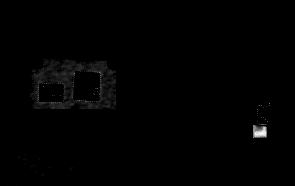
\includegraphics[scale=.7]{tracking/emptyGrid_TRACK2}

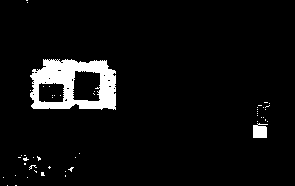
\includegraphics[scale=.7]{tracking/emptyGrid_TRACK}

\end{figure}
\end{frame}

\begin{frame}{Problemer med metoden}
\begin{itemize}
\item Støj
\item Farveændring (lys/skygge)
\item Opdateringshastighed
\end{itemize}

\end{frame}



\begin{frame}{Filtrering af støj}
3x3 Median filter \\


$$w'_{x,y} = \begin{cases}
	0 &\text{hvis } \vert V_{x,y} \vert < \rho \\
	w_{x,y} &\text{hvis } \vert V_{x,y} \vert \geq \rho
\end{cases}$$ \\
hvor $$V_{x,y} = \{w \in N_{x,y} \vert w > 0 \}$$
\end{frame}

\begin{frame}{Farveændring (lys/skygge)}
Løbende opdatering af sporingsfarve.
\begin{figure}
\centering

\includegraphics[scale=.7]{tracking/emptyGrid_FILTER}
\end{figure}

\end{frame}

\begin{frame}{Opdateringshastighed}
\begin{itemize}
\item reducere problemets størrelse.
\item robotten bevæger sig kun korte afstande mellem opdateringer.
\end{itemize}
\end{frame}

\begin{frame}
\begin{figure}
\centering

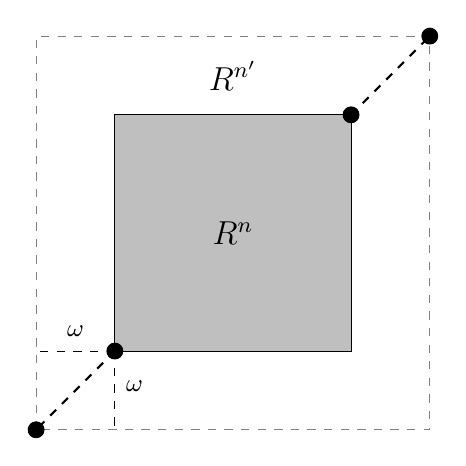
\begin{tikzpicture}[scale=.5]

%set up some coordinates 
%-----------------------
\coordinate (C1) at (0,0); % Outer top left
\coordinate (C2) at (10,10); % Outer bottom right
\coordinate (C3) at (2,2); % Inner top left
\coordinate (C4) at (8,8); % Inner bottom right

%draw figure contents
%--------------------

\draw [fill=lightgray] (C3) rectangle (C4); % Inner rectangle
\draw[dashed, color=gray] (C1) rectangle (C2); % Outer rectangle

\draw [fill] (C1) circle [radius=0.2]; % Outer top right
\draw [fill] (C2) circle [radius=0.2]; % Outer bottom left
\draw [fill] (C3) circle [radius=0.2]; % Inner top right
\draw [fill] (C4) circle [radius=0.2]; % Inner bottom left

\draw[thick,dashed] (C3) -- (C1); % Inner top right to outer top right
\draw[thick,dashed] (C4) -- (C2); % Inner bottom left to outer bottom left

\draw[dashed] (C3) -- (0,2);
\draw[dashed] (C3) -- (2,0);

\draw (5,5) node {\large $R^n$};
\draw (5,9) node {\large $R^{n'}$};

\draw (1,2.5) node {\small $\omega$}; % x1-w
\draw (2.5,1.1) node {\small $\omega$}; % y1-w

\end{tikzpicture}
\end{figure}

\end{frame}

\begin{frame}{Omregning fra punkt i billede til reelt punkt}

Insæt billede der viser ensvinklede trekanter.


\end{frame}









\subsection{Ruteplanlægning}

\begin{frame}{Ruteplanlægning}
Begreber:
\begin{itemize}
\item Destinationscelle
$$D = \{d \in C \vert dest(d) \}$$
\item Synlig celle
$$p(d) = \{e \in C \vert visible(d,e) \}$$
\item Cellens information gain
$$v(d) = \sum_{c \in p(d)}{0.5- \vert 0.5 - P(c) \vert}$$
\end{itemize}

\end{frame}


\begin{frame}

\begin{itemize}
\item Mængde af værdier
$$V = \{v(d) \vert d \in D \}$$
\item Celler med maksimal information gain
$$Q = \{ d \in D \vert v(d) \in maxV \}$$
\item Mængde af distance mellem celler i Q
$$A = \{dist(x,q) \vert q \in Q \}$$
\end{itemize}

\end{frame}

\begin{frame}{Dijkstra's algoritme}

\end{frame}


\section{Design}
\subsection{System Arkitektur}

\begin{frame}{Hardware Komponenter (1)}
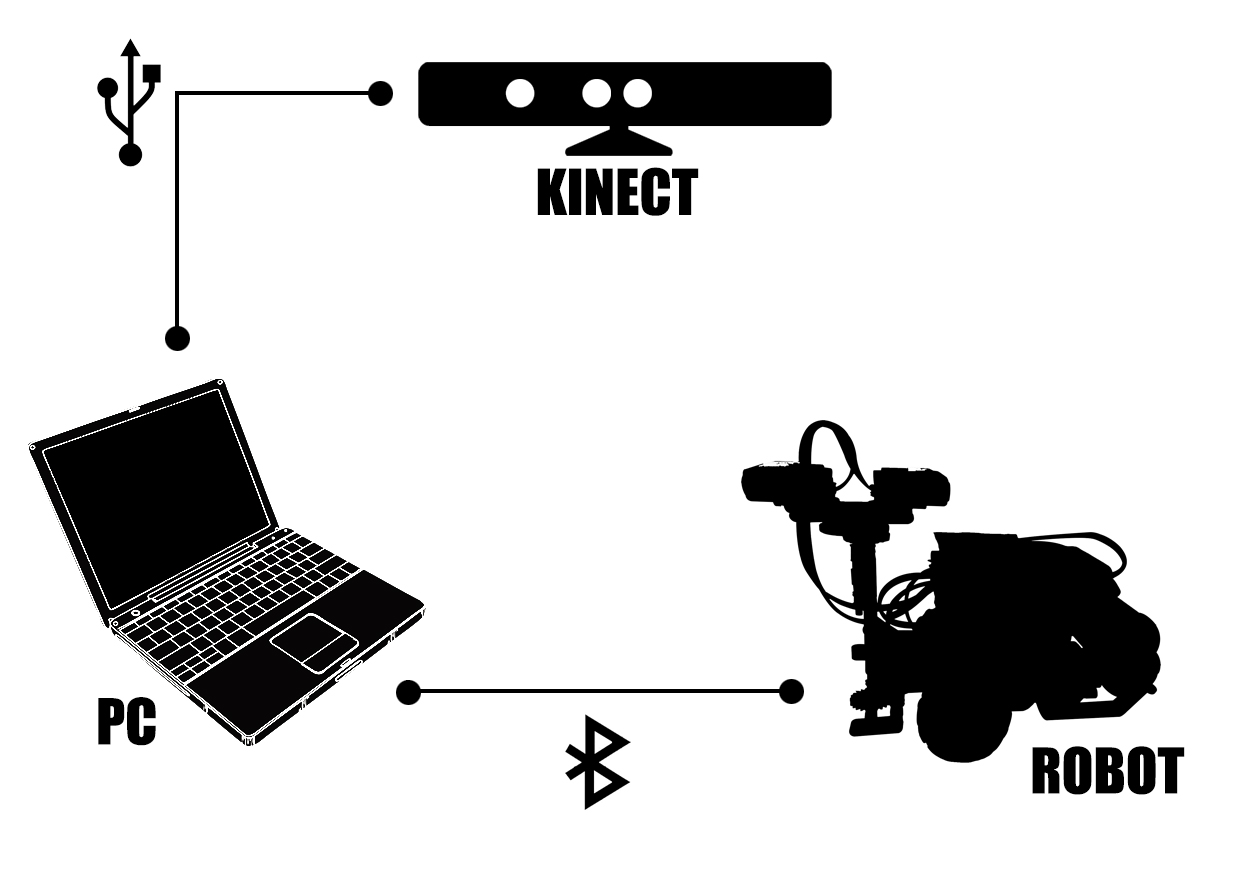
\includegraphics[width=\textwidth]{enheder}
\end{frame}

\begin{frame}{Hardware Komponenter (2)}
\begin{description}
\item[Kinect]{Billed-feed til lokalisering}
\item[NXT]{Navigation i/observation af verden}
\item[PC]{Beregning af:}
\begin{itemize}
\item{kort}
\item{robot lokation}
\item{rute}
\end{itemize}
\end{description}
\end{frame}

\begin{frame}{Hardware Komponenter (3)}
\begin{itemize}
\item{Begrænset anvendelighed;}
\begin{itemize}
\item{Fokus på selve kortlægningen}
\item{God lokationsberegning (afhængig af Kinect)}
\item{Større regnekraft (afhængig af PC)}
\end{itemize}
\end{itemize}
\end{frame}

\subsection{NXT}

\begin{frame}{NXT Software (1)}
3 overordnede filer, med hver deres funktionalitet:
\begin{description}
\item[Sensor.nxc]{Observation af verden}
\item[Navigation.nxc]{Navigation i verden}
\item[Communication.nxc]{Kommunikation med PC}
\end{description}
\end{frame}

\begin{frame}{NXT Software (2)}
\begin{itemize}
\item{Selvstændig (embedded)}
\item{Ingen tunge beregninger}
\item{Gøre op for unøjagtiheder:}
\begin{itemize}
\item{Inkrementerende ''skridt'' ved navigering}
\item{Foretag 2 målinger ved lokation}
\end{itemize}
\end{itemize}
\end{frame}

\subsection{PC}

\begin{frame}{PC Software (1)}
Indsæt overordnet diagram (Yderste komponenter)
\end{frame}

\begin{frame}{PC Software (2)}
\begin{description}
\item[CommonLib]{DTOs, NXTPostMan, Interfaces}
\item[SystemInterface]{GUI og RobotInterface}
\item[Control]{Display, Location og Mapping}
\item[Services]{Robot, Route, Kinect, Tracking}
\item[Data]
\end{description}
\end{frame}

\begin{frame}{PC Software (3)}
\begin{itemize}
\item{Mange processer, samt tunge beregninger:}
\begin{itemize}
\item{Prioritering og samtidighed}
\end{itemize}
\item{Streng/meget arkitektur}
\begin{itemize}
\item{(Fordele/ulemper)}
\end{itemize}
\end{itemize}
\end{frame}

\subsection{Kommunikation}

\begin{frame}{Protokol}
\begin{description}
\item[Generelt]{$< BeskedType >< Indhold >$}
\item[Eksempel 1]{Robot anmoder om lokation\\
\texttt{0}}
\item[Eksempel 2]{PC sender lokation\\
\texttt{\textcolor{red}{52}-0213.5\textcolor{red}{00126.9}00187.4}}
\end{description}
\end{frame}

\begin{frame}{Flow}
Tilstandssekvensdiagram? Komponentdiagram? Vigtigt/spændende?
\end{frame}

\begin{frame}{Sidste tanker}
\end{frame}

Dette kapitel evaluerer de to valgte sensormodeller(\cref{mapping:sensormodel}) og ruteplanlægning(\cref{ruteplanleagning}).


\section{Formål}
Formålet med denne test er at se hvilken sensormodel der kommer frem til det mest præcise kort og hvilken indvirkning ruteplanlægningen har.

\section{Test}\label{evaluering:test_beskrivelse}
Der bliver foretaget tre tests med hver sensormodel(\cref{mapping:sensormodel}).
I alle test benyttes ruteplanlægning beskrevet i \cref{ruteplanlaegning}.
Startpositionen er altid den samme.
Robotten kører hen til et punkt og scanner to gange - dette foretages 75 gange.
Alle data bliver logget så det er muligt at genskabe et kort udfra det.

\subsection{Opstilling}

\subsection{Resultater}

\subsection{Opsummering}
\end{document}